In this section, the results of the main areas this project focused on will be presented. These areas were: a website version of WOLF, a neural network model using TensorFlow, saved models, predictions from models, feature importance, and more benchmark datasets.

\section*{Website}
After setting up and logging into an account on the website, users will be brought to the home screen where information about all activities and components can be seen (Figure \ref{fig:WOLF website home}).

\begin{figure}[H]
	\centering
	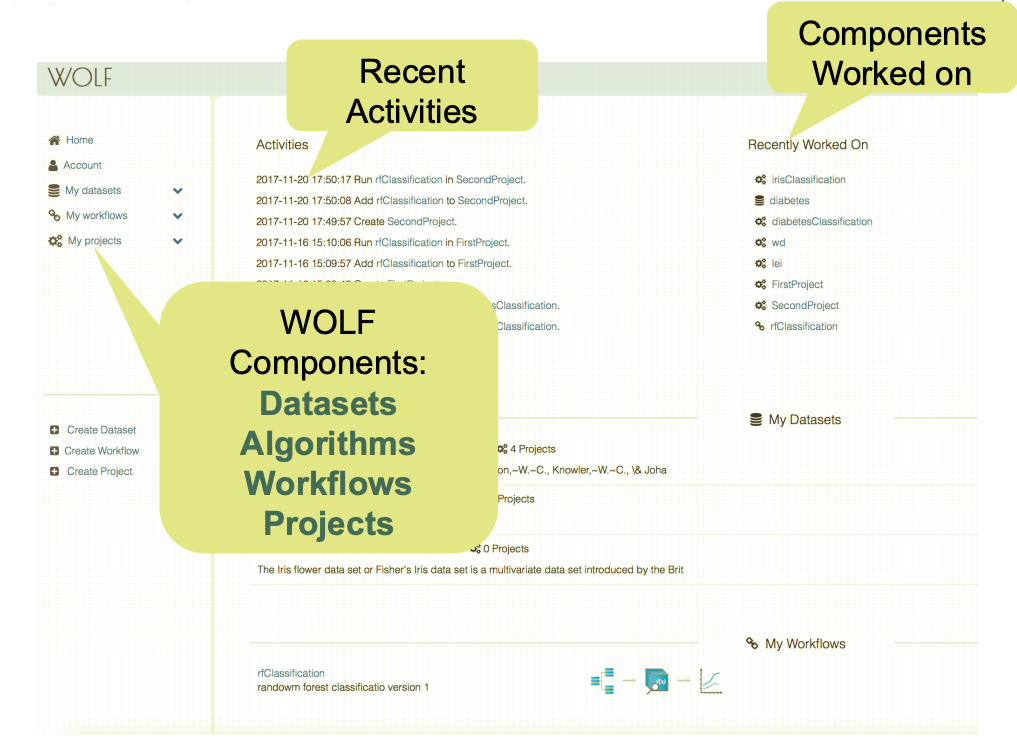
\includegraphics[scale=0.3]{WOLF_home}
	\caption{WOLF homepage \parencite{WOLFpresentation}}
	\label{fig:WOLF website home}
\end{figure}

If a user wants to create a workflow, they are asked to give it a name and a description as well as provide the parameters for each transaction. Figure \ref{fig:WOLF website transaction} shows this, along with the data split transaction.

\begin{figure}[H]
	\centering
	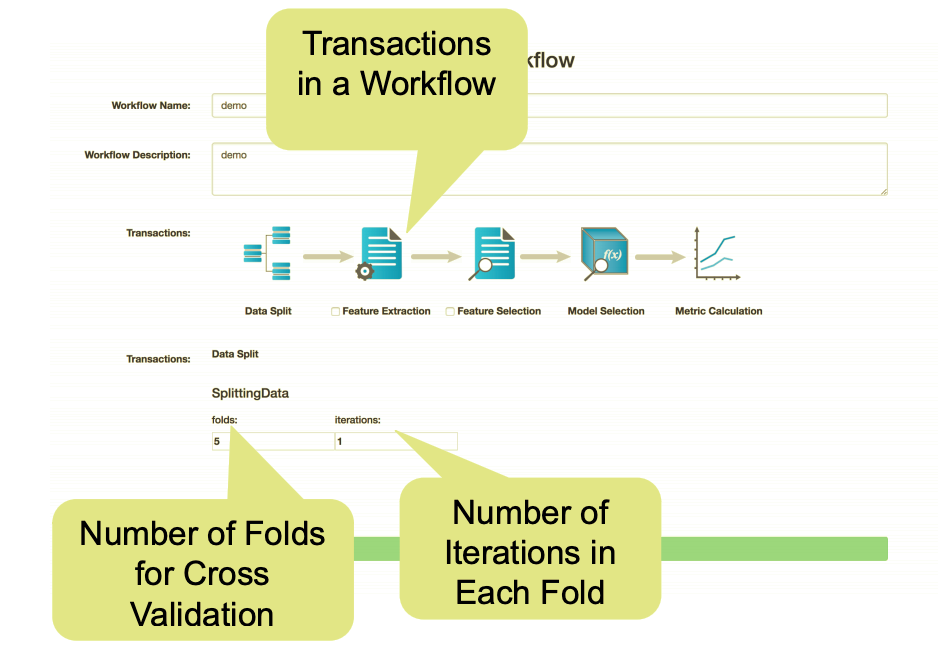
\includegraphics[scale=0.35]{WOLF_transaction}
	\caption{WOLF transactions \parencite{WOLFpresentation}}
	\label{fig:WOLF website transaction}
\end{figure}

The model selection transaction (Figure \ref{fig:WOLF website modelselect}) shows a list of all the possible models to pick from. When the user selects one, it moves to the list on the right and also adds a section below where the hyper-parameters to be tested can be chosen.

\begin{figure}[H]
	\centering
	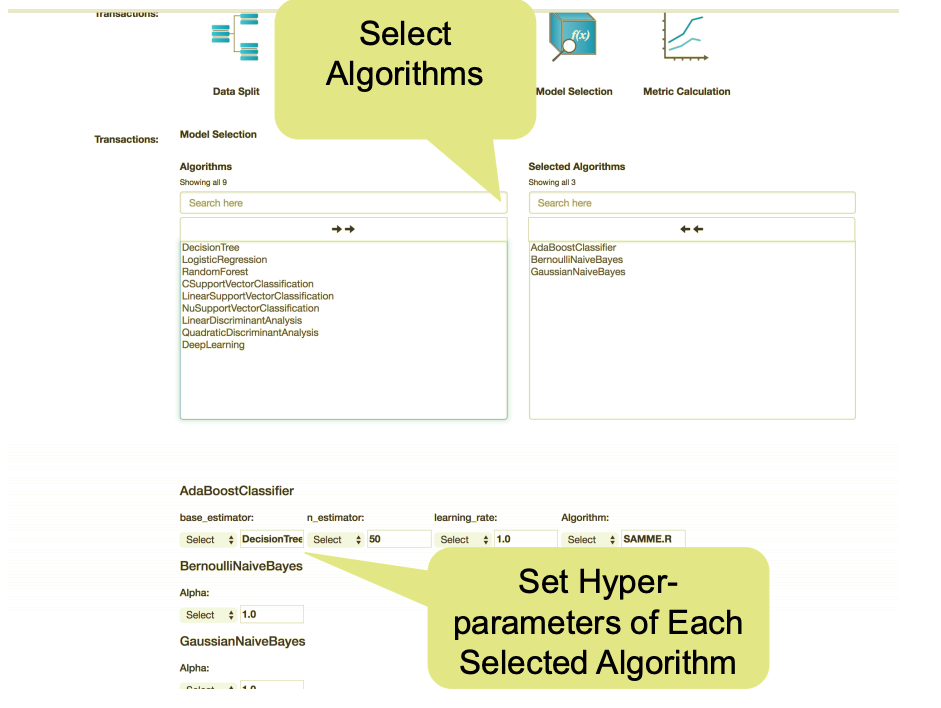
\includegraphics[scale=0.37]{WOLF_modelselect}
	\caption{WOLF models selection \parencite{WOLFpresentation}}
	\label{fig:WOLF website modelselect}
\end{figure}

Once the run of the workflow is completed, the details of the run are shown and a results file can be chosen. This is the one part of the website that currently does not work. But Figure \ref{fig:WOLF website rundetails} shows how it should look when back in a working state. Some of the information shown includes when the job was submitted, when it was completed, the current state of the run, and, most importantly, a link to download the results file.

\begin{figure}[H]
	\centering
	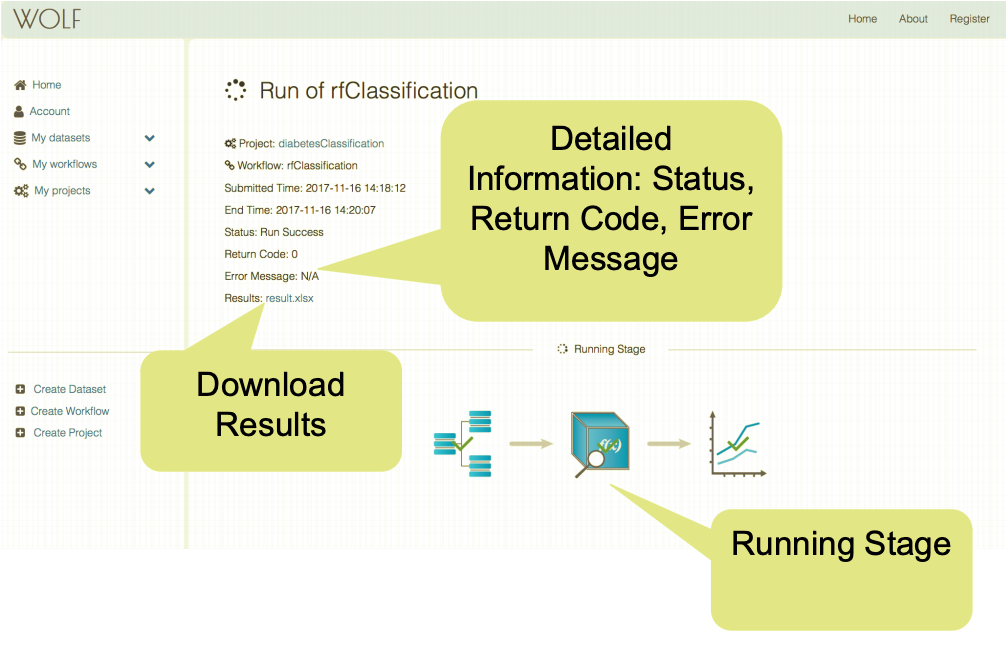
\includegraphics[scale=0.35]{WOLF_rundetails}
	\caption{WOLF run details \parencite{WOLFpresentation}}
	\label{fig:WOLF website rundetails}
\end{figure}

\section*{Neural Network}
The neural network was implemented simply and successfully. Keras was helpful in this and allowed for looping through the number of layers needed and adding each with the provided number of nodes. Then a sequential model is compiled with all of the hyper-parameters. Table \ref{tab:WOLF TF HP} shows all of the hyper-parameters supported and their default values if the user does not provide one. TensorFlow for GPUs is used to run on the ITTC cluster to have faster train times than running on the CPUs. At this time, only one GPU can be used or else it becomes difficult to be assigned nodes and the job becomes stuck waiting in the queue. 
\begin{table}[H]
	\centering
	\begin{tabular}{|l|l|l|}
		\hline
		\textbf{Parameter flag} & \textbf{Description}          & \textbf{Default value}  \\ \hline
		-a             & activation function  & ``relu''       \\ \hline
		-l             & layers               & {[}100,100,100{]} \\ \hline
		-d             & input layer dropout  & 0              \\ \hline
		-h             & hidden layer dropout & 0.5              \\ \hline
		-e             & epochs               & 10             \\ \hline
		-b             & batch size           & None           \\ \hline
		-r             & learning rate        & 0.001          \\ \hline
	\end{tabular}
	\caption{TensorFlow neural network hyper-parameters}
	\label{tab:WOLF TF HP}
\end{table}

\section*{Saved Model and Predictions}
Saving each model to a pickle file creates a different folder of models for each hyper-parameter and model type combination. For each data split, there is one model in the folder. Figure \ref{fig:WOLF saved models} shows the file hierarchy and the list of files for a run with 5 folds.

\begin{figure}[H]
	\centering
	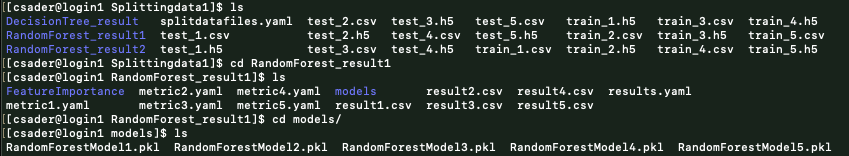
\includegraphics[scale=0.47]{WOLF_models}
	\caption{WOLF saved models}
	\label{fig:WOLF saved models}
\end{figure}

The best model is selected based on the highest metric (ROC-AUC by default) for the chosen model type and hyper-parameter configuration. This best model will have its file path given in the ``best configuration'' tab of the results file that can be seen in Figure \ref{fig:WOLF results}, which was trained on the diabetes dataset.

\begin{figure}[H]
	\centering
	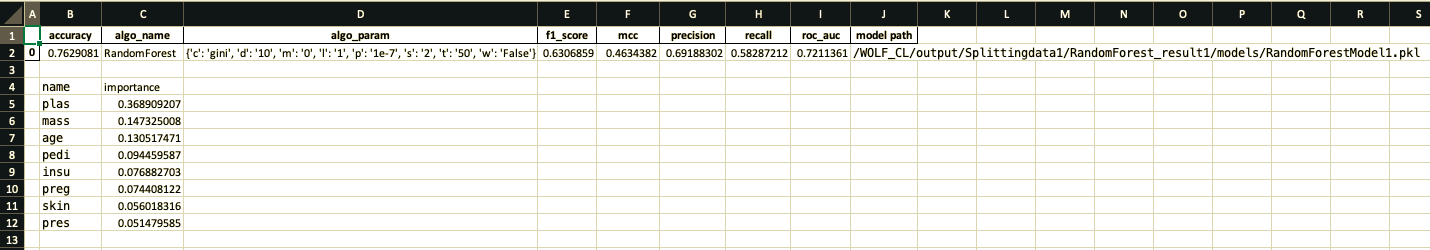
\includegraphics[scale=0.3]{WOLF_results}
	\caption{WOLF results file}
	\label{fig:WOLF results}
\end{figure}

For making predictions, these will be written to a file called {\tt predictions.csv}, which will have as many rows as there were data points to predict. There will only be one column in the file for the class which is to be predicted, but if multi-label classification is added to WOLF, then there will be a column for each label to be predicted.

\section*{Feature Importance}
In calculating feature importance, just like saving models, there will be a folder of feature importances for each model type and hyper-parameter combination. And also just like the models, there is a different file for each data split as each trained model will have different feature importance values. This file hierarchy for a 5 folds data split can be seen in Figure \ref{fig:WOLF feature importances}. The feature importance values for training on the diabetes dataset can be seen in Figure \ref{fig:WOLF results}. The features are sorted by importance.

\begin{figure}[H]
	\centering
	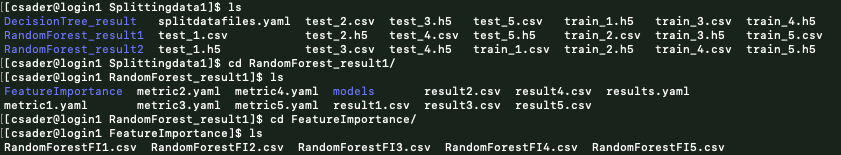
\includegraphics[scale=0.47]{WOLF_importance}
	\caption{WOLF feature importance files}
	\label{fig:WOLF feature importances}
\end{figure}

\section*{Datasets}
WOLF was run on all of the benchmark datasets to test the effectiveness of the workflows. The results for the binary classification datasets can be seen in Table \ref{tab:WOLF benchmark}. All scores are the ROC-AUC values that have been calculated for each model type and each dataset.

\begin{table}[H]
	\centering
	\resizebox{\textwidth}{!}{%
		\begin{tabular}{|c|c|c|c|c|c|c|c|c|c|}
			\hline
			\textbf{Dataset Name}  & \textbf{RF} & \textbf{DT} & \textbf{Lin SVM} & \textbf{Log Reg} & \textbf{BNB} & \textbf{LDA} & \textbf{Ada Boost} & \textbf{NN - Caffe} & \textbf{NN - TF} \\ \hline
			Bank note auth.        & 0.9923      & 0.9810      & 0.9889           & 0.9896           & 0.8419       & 0.9786       & 0.996              & 0.9998              & 0.9999           \\ \hline
			Blood Transfusion      & 0.6279      & 0.5852      & 0.5323           & 0.5495           & 0.4993       & 0.5419       & 0.6181             & 0.5003              & 0.5427           \\ \hline
			Climate Sim. Crashes   & 0.5501      & 0.6527      & 0.7941           & 0.5773           & 0.5000       & 0.7158       & 0.7535             & 0.6581              & 0.7570           \\ \hline
			Sonar, Mines/Rocks     & 0.8167      & 0.6919      & 0.7692           & 0.7507           & 0.5051       & 0.7358       & 0.7954             & 0.6100              & 0.7662           \\ \hline
			Default of credit card & 0.6540      & 0.6081      & 0.5217           & 0.4999           & 0.6731       & 0.6127       & 0.6388             & 0.5000              & 0.5000           \\ \hline
			Fertility              & 0.5531      & 0.4964      & 0.4960           & 0.4988           & 0.5000       & 0.4878       & 0.5375             & 0.5223              & 0.5333           \\ \hline
			Voice Rehabilitation   & 0.7831      & 0.7351      & 0.5058           & 0.5529           & 0.6854       & 0.7256       & 0.7916             & 0.6344              & 0.4934           \\ \hline
			Pima Indians Diabetes  & 0.7216      & 0.6412      & 0.5597           & 0.7151           & 0.5035       & 0.7253       & 0.7131             & 0.6864              & 0.7324           \\ \hline
			Spambase               & 0.9323      & 0.9025      & 0.8252           & 0.9215           & 0.8736       & 0.8699       & 0.9345             & 0.6706              & 0.8887           \\ \hline
			Vertebral Column       & 0.8058      & 0.7592      & 0.7261           & 0.8095           & 0.6438       & 0.8017       & 0.7917             & 0.8101              & 0.7619           \\ \hline
			Wholesale customers    & 0.9053      & 0.8520      & 0.6939           & 0.8765           & 0.5000       & 0.7748       & 0.8800             & 0.5000              & 0.5348           \\ \hline
		\end{tabular}%
	}
	\caption{WOLF benchmark data ROC\_AUC}
	\label{tab:WOLF benchmark}
\end{table}